\documentclass[a4paper,10pt]{article}
\usepackage[top=0.75in, bottom=0.75in, left=0.55in, right=0.85in]{geometry}
\usepackage{graphicx}
\usepackage[latin1]{inputenc}
\usepackage{amsmath}
\usepackage{amsfonts}
\usepackage{amssymb}

\begin{document}

\begin{flushright}
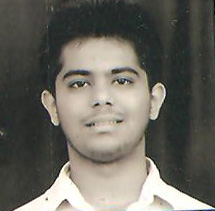
\includegraphics[width=3cm, height=4cm]{001.jpg}\\
\large
\textbf{\bigskip Ayush Bajaj}
\end{flushright}


\begin{flushleft}
	%contact information
	\textbf{\large Contact Information}:\\
	\hrule
	\bigskip
	\textbf{Adress:}            E-42 Dayanand Nagar\\
	\textbf{Contact:}   \texttt{9716989552}\\
	\textbf{Email:}             ayush95bajaj@gmail.com\\
	\bigskip
	\textbf{\large Career Objective} 
	\hrule
	\bigskip
	\textbf{To work in such a manner so that the ease of technology should benifit every common man}
	%education
	\textbf{\large  Education}:\\
	\hrule
	\bigskip
	\begin{tabular}{|c|c|c|c|c|}
   		\hline \textbf{ Degree}  & \textbf{College/school}  & \textbf{University} & \textbf{Passing Year} 			& 		\textbf{ Pass percentage} \\ 
   		\hline B.Tech Electronics & Maharaja Agrasen College  & Delhi University & 2017 & - \\ 
   		\hline 
			10+2 & Delhi Public School Ghaziabad & - & 2013 & 90 \\
    	\hline
\hline 
			10 & Delhi Public School Ghaziabad & - & 2011 & 10 CGPA \\
    	\hline
	\end{tabular} 
	\smallskip
		%projects

		\bigskip
    \textbf{Projects:}\\
    \hrule
	\smallskip
      \begin{enumerate}
      	\item  mine it bot(prototype model for detection of mines in form of boxes)
      	\item  Hand gesture controlled robot using xbee
      	\item  helio bot(prototype of capturing solar energy efficiently by movement of solar panel) 
      \end{enumerate}
      \textbf{Training and Internship:}\\
  \hrule
   \begin{itemize}
   	\item  workshops on embedded systems and robotics\\
   	\item  level 1 cyber security expert\\
   	\item  workshop on fiber optics and optical communications\\
   	\item  workshop on recent trends in semiconductor technology\\
   	\bigskip
   	\textbf{Research Publications:}\\
   	\medskip
  \hrule
 \end{itemize}
  \begin{enumerate}
   \item  presented a paper on solar energy and sustainable development at National Conference held at Maharaja Agrasen College(DU)\\ \medskip
   \end{enumerate}
   \textbf{Technical skills:}\\
  \hrule
   \begin{itemize}
   	\item programming experience in c++,c,embedded c,latex\\
   	\item  Embedded systems\\
   	\item  Android application development\\
   	\item  hardware designing \\
   \item   experience on micro controller based projects\\
    \end{itemize}
    \newpage
     \textbf{Soft skills:}\\
  \hrule
    \begin{enumerate}
    \item innovative\\
    \item keen observer\\
    	\item Good communication skills\\
    	\item Leadership Quality\\
    	\item Teamwork \\
    	\item Adaptability\\
    	\item  desire for learning\\
    	\item positive attitude\\
    \end{enumerate}
    \textbf{Extra Curricular Activities:}\\
  \hrule
  
   
  
  \begin{itemize}
  	\item working for community(member of NSS under leadership development programme )
  \item debating
   \item presenting
  	
  \end{itemize}
\textbf{Co-Curricular Activities:}\\
  \hrule
  
   
  
  \begin{enumerate}
  
 
  	\item sports
  \item music
  	 \end{enumerate}
  	 \textbf{Personal Details:}\\
   \hrule
   
    \begin{itemize}
    	\item Father's Name:     Rajeev Bajaj\\
    	\item Mother's Name:     Dimple Bajaj\\
    	\item Sex:               male\\
    	
    	\item Date of Birth:     9th January 1995 \\
    	\item Nationality:       Indian\\
    	\item Marital Status:    Single\\
    \end{itemize}
     \textbf{ References: }\\
   \hrule
    
    \begin{itemize}
    	\item Dr.Praveen Kant Pandey\\
    	Associate Proffessor(University Of Delhi)\\
    	      Email:pkpandey.du@gmail.com
    	      
     \end{itemize}
     \textbf{ Declaration: }\\
      \hrule
     I hereby declare that all the details furnished above are true to the best of my knowledge and belief.
     \medskip
      
   
	\end{flushleft}
	\end{document}
	